\documentclass[12pt]{report}

% PACKAGE - WHY?
\usepackage{amsmath}    % need for subequations
\usepackage{graphicx}   % need for figures
\usepackage{verbatim}   % useful for program listings
\usepackage{color}      % use if color is used in text
\usepackage{subfigure}  % use for side-by-side figures
\usepackage{hyperref}   % use for hypertext links, including those to external documents and URLs
\usepackage{fancyhdr}   % for image in header
%%%%%%%%%%%%%%%%%%%%%%%%%%%%%%%%%%%%%%%%%%%%%%%%%%%%%%%%%%%%%%%%%%%%%%%%%%%%%%%%%%%%%%%%%%%%%%%%%%%%%%%%%%

% IMMAGINI HEADER
\thispagestyle{fancy}{
\lhead{
\includegraphics[width=4.5cm]{Images/logoUnimi}}
\rhead{
\includegraphics[width=6.5cm]{Images/logoPong}}
}



\begin{document}

% logoTeam
\begin{center}
  \begin{figure}
    \centering
  \vspace*{5\baselineskip}
  
\includegraphics[width=10cm]{Images/logoTeam}
  \end{figure}

  {\large \textbf{Game Title}} \\
  \textbf{\textit{PONG - Game and Level Design}} \\
  {\small Updated 31 October 2018} \\

\begin{tabular}{lcr}\\\\
\textbf{Francesco Periti}    & Francesco.Periti@studenti.unimi.it   & 930650\\
\textbf{Francesco Principe}  & Francesco.Principe@studenti.unimi.it & 937622\\
\textbf{Davide Valentini}    & Davide.Valentini@studenti.unimi.it   & XXX\\
\textbf{Elena Copertchini}   & Elena.Coperchini@gmail.com &\\
\end{tabular}

\end{center}

% CAPITOLO 1 - SINOSSI
\chapter{Synopsis}

Sophie is a brave and inexperienced young witch. She is in love with Howl, a powerful wizard, and they live in a moving castle with a magic door. \par
Howl leaves to complete a mission for the king in the nearby kingdom of Strangia in order to stop the war. Weeks later, giving that the war is still going on, she gets worried and she starts looking for him. \par
Using the magic door, she gets to the capital of Strangia along with her friend Calcifer, a fire demon. They don’t find Howl, but they save prince Justin, an old friend of their, who has been imprisoned by Mizar, his stepmother and the current ruler of Strangia. \par
Mizar is a djinn and sha has been imprisoned Howl in the reign of spirits. In order to save him, Sophie and Calcifer ask another djinn for help to enter into the reign of spirits. \par
They save Howl and they find a way to defeat her. \par
Sophie, Calcifer and Howl face Mizar and they overcome her.



% CAPITOLO 1 - SINOSSI
\chapter{Goals outline}

\section{Train in the castle}
\begin{enumerate}
\item talk to objects in the moving castle
\item explore the moving castle
\item learn how to sew magic hats
\end{enumerate}

\section{Find out what happened to Howl}
\begin{enumerate}
\item go to Kingsbury
\item go see Suliman
\item fight enemies
\item go back to moving castle
\end{enumerate}

\section{Look for Howl}
\begin{enumerate}
\item go to the capital of Strangia
\item talk with a beggar
\item look for Justin
\item free Justin
\item go back to Suliman with Justin
\end{enumerate}

\section{Go to Belzel}
\begin{enumerate}
\item talk to Suliman
\item go to the desert in the south of Ingary with the moving castle
\item find Belzel’s home
\item persuade Belzel to open a gate to the world of spirits
\end{enumerate}

\section{Free Howl}
\begin{enumerate}
\item enter the world of spirits
\item defeat enemies and solve puzzles
\item find Howl and save him
\item go back to moving castle
\end{enumerate}

\section{Defeat Mizar}
\begin{enumerate}
\item use black sector with Howl to see Mizar’s past
\item go to the hideout of Mizar’s heart
\item go through the dungeon and reach Mizar’s heart
\item defeat Mizar
\item choose to kill Mizar or spare her
\end{enumerate}


% CAPITOLO 1 - PERSONAGGI
\chapter{Characters}
% SCEGLIETE PURE VOI L'ORDINE {TODO}

  \section{Sophie Hatter}

\textbf{Name}: Sophie Hatter \\
\textbf{Function}: Hero, protagonist

\subsection{Internal World}

\textbf{Age \& Gender}: 19, Female \\
\textbf{Values \& Virtues}: Brave, loyal, friendly \\
\textbf{Personality}: Optimistic, intelligent, altruist, impulsive, compassionate \\
\textbf{Interests}: Hats, Magic \\
\textbf{Ethnic Group}: Human, Witch

\subsection{External World}
\textbf{Environment}: Wastelands, Howl’s Moving Castle \\
\textbf{Education}: Average-education \\
\textbf{Social \& Cultural Background}: Middle Class family \\
\textbf{Look \& Feel}: Her hair is white and looks like an old woman’s but she is a beautiful young girl. Generally she wears long dress. She loves to sew and wear hats \\
\textbf{Job \& Experience}: Cleaning woman, Hatter \\
\\
\textbf{Relatives \& Relation}:
\begin{enumerate}
\item \textbf{Howl}: She is in love with him, her partner. She lives with him in The Moving Castle with Calcifer
\item \textbf{Calcifer}: He his her friend and lives with her in The Moving Castle
\item \textbf{Justin}: Justin is her old friend who makes her meet Howl for the first time
\item \textbf{Suliman}: She respects Suliman as great magician and due to this fact she trusts her
\item \textbf{Mizar}: At the beginning she doesn’t know him. She is in conflict with her since she 
apprehends that Mizar has trapped Howl
\item \textbf{Belzel}: At the beginning she doesn’t know him. He is her last hope to rescue Howl from the reign of spirits
\end{enumerate}

\subsection{Description}
Sophie is brave and altruist girl. She represents the Hero of the Story who is going to save Howl. She is also optimistic but she always worries about her beloved ones. She hasn’t lost the passion for hats and occasionally she sews one.

\subsection{Background story}
Before She fell in love with Howl She lived in the small town within the Kingdom of Ingary. She is the eldest of two sisters and aimed to become a hatter like her father. After the misadventure of the curse launched by the Wastelands Witch, she has discovered being a which. Her white hair is the sign of the passed curse. Her magic powers lets her speak with some objects but she is a novice and she has to learn almost everything about the magic world.


  \section{Howl}

\textbf{Name}: Howl Jenkins Pendragon \\
\textbf{Function}: Victim who has to be rescued first, helper during the final fight then

\subsection{Internal World}

\textbf{Age \& Gender}: 27-30, Male \\
\textbf{Values \& Virtues}: Beauty \\
\textbf{Personality}: Friendly, passionate, emotive, lazy, leader \\
\textbf{Interests}: Magic, body care \\
\textbf{Ethnic Group}: Wizard, Human

\subsection{External World}
\textbf{Environment}: Wastelands, Howl’s Moving Castle \\
\textbf{Education}: High-education \\
\textbf{Social \& Cultural Background}: He has always been famous as one of the most powerful wizards of Ingary \\
\textbf{Look \& Feel}: Young handsome man   \\
\textbf{Job \& Experience}: Experienced wizard \\
\\
\textbf{Relatives \& Relation}:
\begin{enumerate}
\item \textbf{Sophie}: He is in love with her, his partner. He lives with her in the Moving Castle
        with Calcifer
\item \textbf{Calcifer}: He is a long-time friend of him and live with him in the Moving Castle
\item \textbf{Justin}: They barely know each other
\item \textbf{Suliman}:He has a great respect for Suliman, his magic teacher
             He is slightly submissive to her and really takes into consideration what she says
\item \textbf{Mizar}: He hates her because she wants the war to go on and because she trapped him into an inescapable prison 
\item \textbf{Belzel}: No one knows each other
\end{enumerate}

\subsection{Description}
Howl is a powerful Wizard that works as an emissary for the Kingdom of Ingary. In the story he has to be rescued from the Mizar’s trap. He know every secret of the Moving Castle and he is the only one who can transform and edit it.

\subsection{Background story}
Howl is always being notorious as a powerful wizard of Ingary. After that the pact with Calcifer has been broken, he decided to introduce and train Sophie in magic. He created a magic needle that she can use to sew magic hats. Before leaving for the mission he also created a magic lantern for Calcifer. Calcifer, free from the pact, can go out the castle inside the lantern without the Moving Castle being destroyed. Suliman gave him the mission to stop the war, but he disappeared.




  \section{Mizar}

\textbf{Name}: Mizar\\
\textbf{Function}: The Antagonist, The Evil Stepmother

\subsection{Internal World}

\textbf{Age \& Gender}: 200, Female \\
\textbf{Values \& Virtues}: Vengeance \\
\textbf{Personality}: Manipulator, Heartless, Egocentric, vindictive \\
\textbf{Interests}: Magic, King of Ingary \\
\textbf{Ethnic Group}: Djinn, Arabic

\subsection{External World}
\textbf{Environment}: The castle of the Kingdom of Strangia. \\
\textbf{Education}: High-educated \\
\textbf{Social \& Cultural Background}: Each people in Strangia respects her because they fear her power. Nobody knows the real reasons why the war is going on. Nobody knows the real story of Mizar \\
\textbf{Look \& Feel}: Her age is 200 but she looks like a 30-35 years old woman. She has pointy ears  \\
\textbf{Job \& Experience}: Court Magician, Queen regent \\
\\
\textbf{Relatives \& Relation}: Every relation she has is just submission to her.
\begin{enumerate}
\item \textbf{Sophie}: She didn’t know Sophie until she tries to defeat her. Since then, Mizar hates her.
\item \textbf{Howl}: She knows him just by reputation but she has never met him until he tries to defeat her. Since then, Mizar hates him. She fears him a bit because rumors say that he is a great wizard.
\item \textbf{Calcifer}: She hates him because he is a friend of Sophie and Howl.
\item \textbf{Belzel}: She doesn’t know him.
             He is slightly submissive to her and really takes into consideration what she says
\item \textbf{Justine}: He is her stepson. She gets him arrested only because he is a bare  inconvenient with her plans. 
\item \textbf{Suliman}:Mizar has only heard about her, but she still hates her because it’s the new magician of the king of Ingary.
\end{enumerate}

\subsection{Description}
Before being refused, she was the court magician at castle of Ingary. Since she left the castle, she doesn't have any other interest except avenging the humiliation suffered from the king.
She aims to become the most powerful Djinn of the kingdom because she wants to take revenge of the King of Ingary. According to this, she is willing to do anything to make the war go on.

\subsection{Background story}
Her past is unknown.In fact, She is too old for all of the humans beings and nobody knows her story except some of the most recent ones. A long time ago she worked as court magician of the Kingdom of Ingary. She fell in love with the King she declared her love to him, but without the expected results. In fact, the King mocked her and told her he could never love a djinn. She felt humiliated and decided to make him pay for it. She tore out her heart with a spell in order to end her suffering and hid it in a secret place. This act increased his hatred and desire for revenge. Using another spell she charms the king of Strangia and she tricks him in marrying her.




  \section{Belzel}

\textbf{Name}: Belzel \\
\textbf{Function}: Helper

\subsection{Internal World}

\textbf{Age \& Gender}: 347, Male \\
\textbf{Values \& Virtues}: Man of his word  \\
\textbf{Personality}: Quiet, loner, helpful, kind \\
\textbf{Interests}: Meditation, inner peace \\
\textbf{Ethnic Group}: Arabic Djinn

\subsection{External World}
\textbf{Environment}: Desert in the South of Ingary.  \\
\textbf{Education}: High-educated. \\
\textbf{Social \& Cultural Background}: He has left society many decades ago and he is used to live alone. \\
\textbf{Look \& Feel}: He looks like a 50-years-old fat man with long beard. \\
\textbf{Job \& Experience}: He is a powerful wizard. \\
\\
\textbf{Relatives \& Relation}:
\begin{enumerate}
\item \textbf{Sophie and Calcifer}: He  is glad to help them because he feels they really need his help.
\item \textbf{Howl, Justine, Mizar}: No one knows each other
\item \textbf{Suliman}: He doesn’t know her
\end{enumerate}

\subsection{Description}
He is a djinn who spends his days meditating and practicing with new spells, he loves being helpful for people who actually need his help. 


\subsection{Background story}
He decided to move centuries ago into the desert because he felt like the society he was living in was too selfish and asked him for help only for futile things 
Nowadays, no one knows him personally but people in the southern kingdom think, according to a common legend that survived across the centuries, he still lives alone in the desert and he can help you when you are really in trouble.




  \section{Calcifer}

\textbf{Name}: Howl Jenkins Pendragon \\
\textbf{Function}: Victim who has to be rescued first, helper during the final fight then

\subsection{Internal World}

\textbf{Age \& Gender}: 27-30, Male \\
\textbf{Values \& Virtues}: Beauty \\
\textbf{Personality}: Friendly, passionate, emotive, lazy, leader \\
\textbf{Interests}: Magic, body care \\
\textbf{Ethnic Group}: Wizard, Human

\subsection{External World}
\textbf{Environment}: Wastelands, Howl’s Moving Castle \\
\textbf{Education}: High-education \\
\textbf{Social \& Cultural Background}: He has always been famous as one of the most powerful wizards of Ingary \\
\textbf{Look \& Feel}: Young handsome man   \\
\textbf{Job \& Experience}: Experienced wizard \\
\\
\textbf{Relatives \& Relation}:
\begin{enumerate}
\item \textbf{Sophie}: He is in love with her, his partner. He lives with her in the Moving Castle
        with Calcifer
\item \textbf{Calcifer}: He is a long-time friend of him and live with him in the Moving Castle
\item \textbf{Justin}: They barely know each other
\item \textbf{Suliman}:He has a great respect for Suliman, his magic teacher
             He is slightly submissive to her and really takes into consideration what she says
\item \textbf{Mizar}: He hates her because she wants the war to go on and because she trapped him into an inescapable prison 
\item \textbf{Belzel}: No one knows each other
\end{enumerate}

\subsection{Description}
Howl is a powerful Wizard that works as an emissary for the Kingdom of Ingary. In the story he has to be rescued from the Mizar’s trap. He know every secret of the Moving Castle and he is the only one who can transform and edit it.

\subsection{Background story}
Howl is always being notorious as a powerful wizard of Ingary. After that the pact with Calcifer has been broken, he decided to introduce and train Sophie in magic. He created a magic needle that she can use to sew magic hats. Before leaving for the mission he also created a magic lantern for Calcifer. Calcifer, free from the pact, can go out the castle inside the lantern without the Moving Castle being destroyed. Suliman gave him the mission to stop the war, but he disappeared.




  \section{Justine}

\textbf{Name}: Howl Jenkins Pendragon \\
\textbf{Function}: Victim who has to be rescued first, helper during the final fight then

\subsection{Internal World}

\textbf{Age \& Gender}: 27-30, Male \\
\textbf{Values \& Virtues}: Beauty \\
\textbf{Personality}: Friendly, passionate, emotive, lazy, leader \\
\textbf{Interests}: Magic, body care \\
\textbf{Ethnic Group}: Wizard, Human

\subsection{External World}
\textbf{Environment}: Wastelands, Howl’s Moving Castle \\
\textbf{Education}: High-education \\
\textbf{Social \& Cultural Background}: He has always been famous as one of the most powerful wizards of Ingary \\
\textbf{Look \& Feel}: Young handsome man   \\
\textbf{Job \& Experience}: Experienced wizard \\
\\
\textbf{Relatives \& Relation}:
\begin{enumerate}
\item \textbf{Sophie}: He is in love with her, his partner. He lives with her in the Moving Castle
        with Calcifer
\item \textbf{Calcifer}: He is a long-time friend of him and live with him in the Moving Castle
\item \textbf{Justin}: They barely know each other
\item \textbf{Suliman}:He has a great respect for Suliman, his magic teacher
             He is slightly submissive to her and really takes into consideration what she says
\item \textbf{Mizar}: He hates her because she wants the war to go on and because she trapped him into an inescapable prison 
\item \textbf{Belzel}: No one knows each other
\end{enumerate}

\subsection{Description}
Howl is a powerful Wizard that works as an emissary for the Kingdom of Ingary. In the story he has to be rescued from the Mizar’s trap. He know every secret of the Moving Castle and he is the only one who can transform and edit it.

\subsection{Background story}
Howl is always being notorious as a powerful wizard of Ingary. After that the pact with Calcifer has been broken, he decided to introduce and train Sophie in magic. He created a magic needle that she can use to sew magic hats. Before leaving for the mission he also created a magic lantern for Calcifer. Calcifer, free from the pact, can go out the castle inside the lantern without the Moving Castle being destroyed. Suliman gave him the mission to stop the war, but he disappeared.




  \section{Suliman}

\textbf{Name}: Sophie Hatter \\
\textbf{Function}: Hero, protagonist

\subsection{Internal World}

\textbf{Age \& Gender}: 19, Female \\
\textbf{Values \& Virtues}: Brave, loyal, friendly \\
\textbf{Personality}: Optimistic, intelligent, altruist, impulsive, compassionate \\
\textbf{Interests}: Hats, Magic \\
\textbf{Ethnic Group}: Human, Witch

\subsection{External World}
\textbf{Environment}: Wastelands, Howl’s Moving Castle \\
\textbf{Education}: Average-education \\
\textbf{Social \& Cultural Background}: Middle Class family \\
\textbf{Look \& Feel}: Her hair is white and looks like an old woman’s but she is a beautiful young girl. Generally she wears long dress. She loves to sew and wear hats \\
\textbf{Job \& Experience}: Cleaning woman, Hatter \\
\\
\textbf{Relatives \& Relation}:
\begin{enumerate}
\item \textbf{Howl}: She is in love with him, her partner. She lives with him in The Moving Castle with Calcifer
\item \textbf{Calcifer}: He his her friend and lives with her in The Moving Castle
\item \textbf{Justin}: Justin is her old friend who makes her meet Howl for the first time
\item \textbf{Suliman}: She respects Suliman as great magician and due to this fact she trusts her
\item \textbf{Mizar}: At the beginning she doesn’t know him. She is in conflict with her since she 
apprehends that Mizar has trapped Howl
\item \textbf{Belzel}: At the beginning she doesn’t know him. He is her last hope to rescue Howl from the reign of spirits
\end{enumerate}

\subsection{Description}
Sophie is brave and altruist girl. She represents the Hero of the Story who is going to save Howl. She is also optimistic but she always worries about her beloved ones. She hasn’t lost the passion for hats and occasionally she sews one.

\subsection{Background story}
Before She fell in love with Howl She lived in the small town within the Kingdom of Ingary. She is the eldest of two sisters and aimed to become a hatter like her father. After the misadventure of the curse launched by the Wastelands Witch, she has discovered being a which. Her white hair is the sign of the passed curse. Her magic powers lets her speak with some objects but she is a novice and she has to learn almost everything about the magic world.


  
  \begin{figure}
    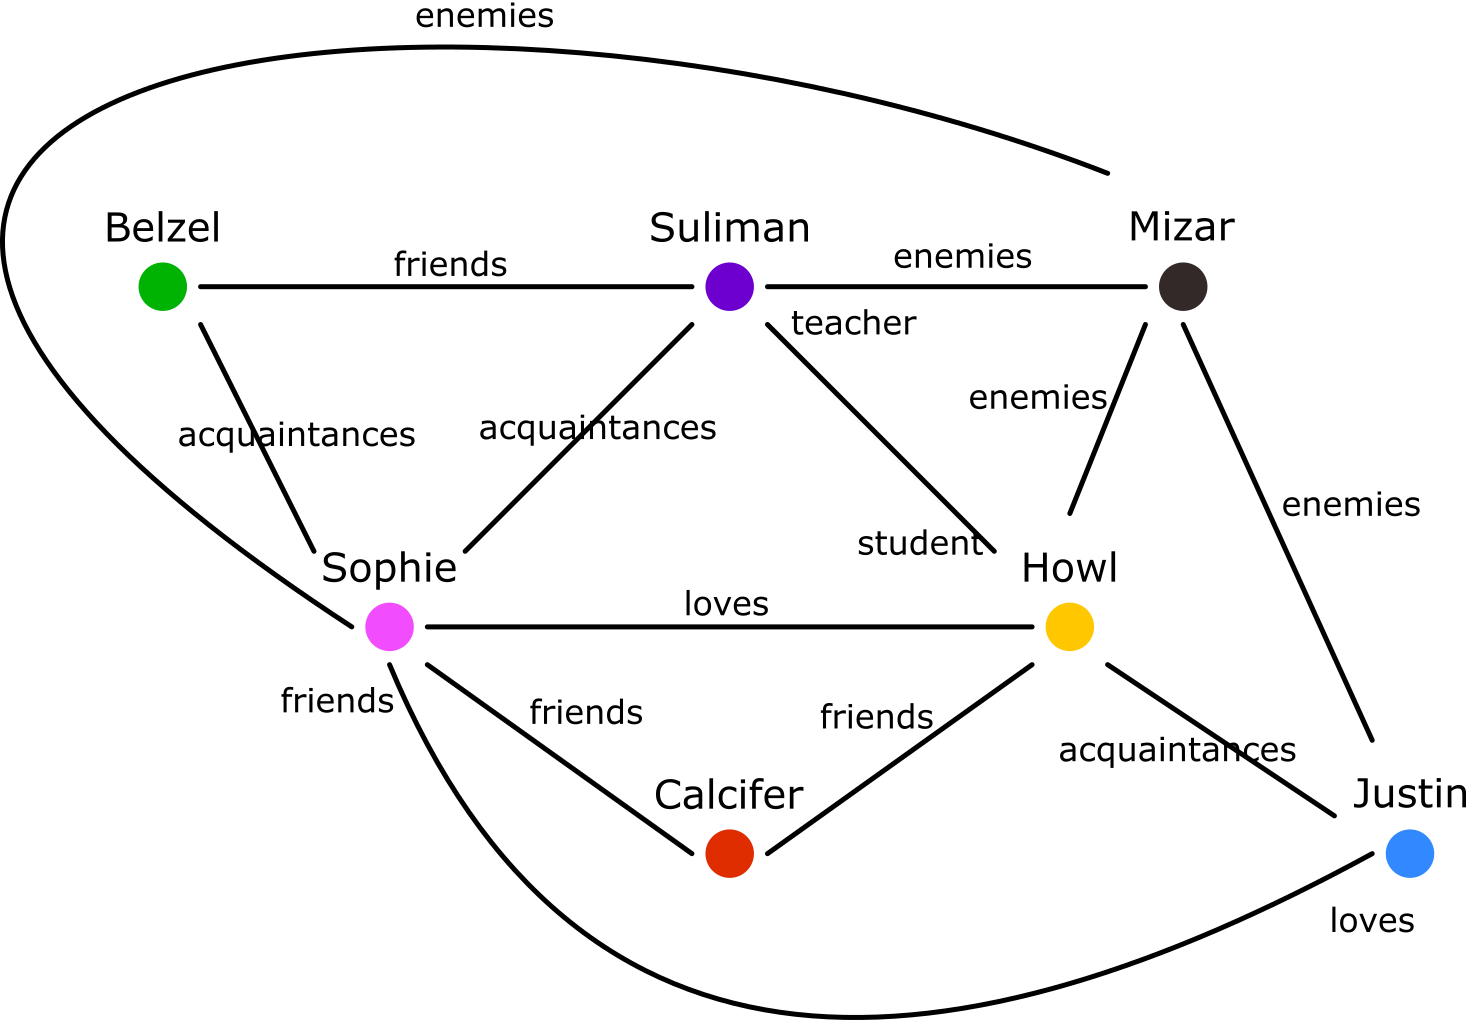
\includegraphics[scale=0.35]{images/relationships}
    \caption{Graph of relationships}
  \end{figure}


  

\end{document}
